
\documentclass[preprint,12pt]{elsarticle}

\usepackage[spanish]{babel}
\usepackage{amssymb}
\usepackage{graphicx}
\usepackage{lineno}
\usepackage[utf8]{inputenc}
\usepackage{url}
\usepackage{color}
\usepackage{enumerate} 
\usepackage[hidelinks]{hyperref}


\begin{document}
	
	\begin{frontmatter}
		
		
		\title{\huge Sistema de Recomendación de Libros de Biblioteca}
		\author{Mamani Ayala, Brandon        (2015052715)}
		\author{Quispe Mamani, Angelo	      (2015052826)}
		\author{Vizcarra Llanque, Jhordy	      (2015052719)}
		\author{Ordoñez Quilli, Ronald          (2015052821)}
		\author{Rodriguez Mamani, Juan      (2017057862)}
		
		\address{Tacna, Perú}
		
		\begin{abstract}
			%% Text of abstract
			
The recommendation systems are part of an information filtering system, which present different types of topics or information items (movies, music, books, news, images, web pages, etc.) that are of interest to a user. particular. In this short article we will try to provide a general explanation about the different data models, such as Content Filtering and Collaborative Filtering.
Then we will apply these models in an example with the help of Colab, where we will filter data and show the results as well as their different graphs.
Then we will give some appreciations and conclusions of what was our Final Work.\\
		\end{abstract}
\end{frontmatter}
%%

	
	%%
	%\linenumbers
	
	%% main text
	\section{Resumen}
Los sistemas de recomendación forman parte de un sistema de filtrado de información, los cuales presentan distintos tipos de temas o ítems de información (películas, música, libros, noticias, imágenes, páginas web, etc.) que son del interés de un usuario en particular. En este breve artículo intentaremos brindar una explicación general acerca de los diferentes modelos de datos, tales como el Filtrado por Contenido y Filtrado Colaborativo.
Luego se aplicarán dichos modelos en un ejemplo con ayuda de Colab, donde filtraremos datos y mostraremos los resultados así como sus diferentes gráficas.
Luego daremos unas apreciaciones y conclusiones de lo que fue nuestro Trabajo Final.\\
	%%
	
	%%
	%\linenumbers
	
	%% main text

\section{Introduccion}

Todos hemos estado expuestos a los famosos “filtros colaborativos”: cuando estabas comprando online y automáticamente el sitio web te recomienda otro artículo similar, o cuando le diste “me gusta” a algo y de repente te empezaron a salir recomendaciones similares en una red social. Los sistemas de recomendación evalúan patrones de tu comportamiento y de miles de usuarios a la vez para emitir nuevas recomendaciones. Ésta es una de las aplicaciones más comunes de “Machine Learning”, porque te da la sensación de estar navegando en un sitio web programado únicamente para tí.

La mayoría de sistemas de recomendación de productos usan filtros colaborativos. Estamos en una era donde nosotros como usuarios generamos más información que nunca antes en la historia. Esta información es usada por los servicios que usamos a diario para darnos una experiencia mas personalizada.

Un claro ejemplo de esto es Netflix, ellos usan la información que nosotros generamos para hacernos recomendaciones y mostrarnos categorías y películas según nuestros gustos. Otro ejemplo es Amazon, que hace recomendaciones de productos que nos podrían interesar, basándose en los productos que ya compramos.

El filtro colaborativo es una técnica usada por los sistemas de recomendación, se basa en el hecho de que si dos personas X y Y en un mismo sistema tienen gustos similares, entonces recomendarle a la persona X cosas que le gusten a la persona Y será de gran relevancia, en contraste a simplemente darle una opción cualquiera.

Hay una variación de filtro colaborativo que se basa en comparar los items en vez de los usuarios para arrojar los items relacionados, de modo que si un usuario entra a ver un determinado item, le podemos recomendar otro.\\

\pagebreak
	%%
	
	%%
	%\linenumbers
	
	%% main text

\section{Marco Teorico}

\begin{enumerate}[3.1]
    \item Introduccion. \\
\\
Un almacen de datos (data warehouse, DW) segun Inmon (Inmon 02, Imhoff y Galemmo 03), es una colecci\'on de datos orientada a un determinado \'ambito (empresa, organización, etc.), integrado, no volátil y variable en el tiempo, que ayuda a la toma de decisiones en la entidad en la que se utiliza. Se trata, sobre todo, de un historial completo de la organización, más allá de la información transaccional y operacional, almacenado en una base de datos diseñada para favorecer el análisis y la divulgación eficiente de datos (especialmente con herramientas OLAP, de procesamiento analítico en línea). Por otra parte Kimball (Kimball 98) la define como “una copia de los datos transaccionales estructurados específicamente para consultas y analisis”. Actualmente uno de los mayores impedimentos para construir este tipo de almacenes de datos es la falta de conocimiento de metodologías adecuadas para su implementación, y la disciplina para cumplirlas. En este breve art\'iculo describiremos la metodología más utilizada actualmente: la metodología de Kimball.

    \item Metodologias Actuales \\
\\
 Existen muchas metodologías de diseño y construcción de DW. Cada fabricante de software de inteligencia de negocios busca imponer una metodología con sus productos. Sin embargo, se imponen entre la mayoría dos metodologías, la de Kimball y la de Inmon. Para comprender la mayor diferencia entre estas dos metodologías, debemos explicar además de la noción de DW mencionando en la introducción, la idea de Data mart. Un Data mart (Kimball et al 98) es un repositorio de información, similar a un DW, pero orientado a un área o departamento específico de la  organización (por ejemplo Compras, Ventas, RRHH, etc.), a diferencia del DW que cubre toda la organización, es decir la diferencia fundamental es su alcance.
Desde el punto de vista arquitectónico, la mayor diferencia entre los dos autores es el sentido de la construcción del DW, esto es comenzando por los Data marts o ascendente (Bottom-up, Kimball) o comenzando con todo el DW desde el principio, o descendente.
Por otra parte, la metodología de Inmon se basa en conceptos bien conocidos del diseño de bases de datos relacionales (Inmon 02, Imhoff y Galemmo 03) la metodología para la construcción de un sistema de este tipo es la habitual para construir un sistema de información, utilizando las herramientas habituales, al contrario de la de Kimball, que se basa en un modelado dimensional (no normalizado)


    \item Metodologia Inmon \\
\\
Bill Inmon ve la necesidad de transferir la información de los diferentes OLTP (Sistemas Transaccionales) de las organizaciones a un lugar centralizado donde los datos puedan ser utilizados para el analisis (sería el CIF o Corporate Information Factory).\\
 Insiste ademas en que ha de tener las siguientes características:
\begin{itemize}
		\item Orientado a temas: Los datos en la base de datos están estructurados de forma que los datos estén relacionados.
		\item Integrado: La base de datos contiene los datos de todos los sistemas operacionales de la organización, y dichos datos deben ser consistentes.
		\item No volátil: La información no se modifica ni se elimina, una vez almacenado un dato, éste se convierte en información de sólo lectura, y se mantiene para futuras consultas.
		\item Variante en el tiempo: Los datos que sufren un cambio a través del tiempo, deben ser registrados para que los informes generados reflejen esas variaciones.
\end{itemize}

La información ha de estar a los máximos niveles de detalle. Los Dw departamentales o datamarts son tratados como subconjuntos de este Dw corporativo, que son construidos para cubrir las necesidades individuales de analisis de cada departamento, y siempre a partir de este Dw Central (del que también se pueden construir los ODS ( Operational Data Stores ) o similares).\\


El enfoque Inmon tambien se referencia normalmente como Top-down. Los datos son extraidos de los sistemas operacionales por los procesos ETL y cargados en las areas de stage, donde son validados y consolidados en el DW corporativo, donde ademas existen los llamados metadatos que documentan de una forma clara y precisa el contenido del DW. Una vez realizado este proceso, los procesos de refresco de los Data Mart departamentales obtienen la información de el, y con las consiguientes transformaciones, organizan los datos en las estructuras particulares requeridas por cada uno de ellos, refrescando su contenido.\\

\begin{itemize}
		\item Definición de Data Warehouse: Un Data Warehouse proporciona una visión global, común e integrada de los datos de la organización, independiente de cómo se vayan a utilizar posteriormente por los consumidores o usuarios. Normalmente en el almacén de datos habrá que guardar información histórica que cubra un amplio período de tiempo. \\
		\item Definición de Data Mart: Podemos entender un Data Mart como un subconjunto de los datos del Data Warehouse con el objetivo de responder a un determinado análisis, función o necesidad y con una población de usuarios específica. Al igual que en un data warehouse, los datos están estructurados en modelos de estrella o copo de nieve y un data mart puede ser dependiente o independiente de un data warehouse. \\
\end{itemize}



    \item Metodologia Kimball en detalle.\\
\\

La metodología se basa en lo que Kimball denomina Ciclo de Vida Dimensional del Negocio (Business Dimensional Lifecycle) (Kimball et al 98, 08, Mundy y Thornthwaite 06). Este ciclo de vida del proyecto de DW, está basado en cuatro principios básicos :
\begin{itemize}
  \item Centrarse en el negocio:  Hay que concentrarse en la identificación de los requerimientos del negocio y su valor asociado, y usar estos esfuerzos para desarrollar relaciones sólidas con el negocio, agudizando el análisis del mismo y la competencia consultiva de los implementadores.
\\
  \item Construir una infraestructura de informaci\'on adecuada: Diseña una base de información única, integrada, fácil de usar, de alto rendimiento donde se reflejará la amplia gama de requerimientos de negocio identificados en la empresa.\\
  \item Realizar entregas en incrementos significativos crear el almacén de datos (DW) en incrementos entregables en plazos de 6 a 12 meses. Hay que usa el valor de negocio de cada element identificado para determinar el orden de aplicación de los incrementos. En esto la metodología se parece a las metodologías ágiles de construcción de software.\\
  \item 
Ofrecer la solución completa proporcionar todos los elementos necesarios para entregar valor a los usuarios de negocios. Para comenzar, esto significa tener un almacén de datos sólido, bien diseñado, con calidad probada, y accesible. También se deberá entregar herramientas de consulta ad hoc, aplicaciones para informes y análisis. \\
\end{itemize} 



La construcción de una solución de DW/BI (Datawarehouse/Business Intelligence) es sumamente compleja, y Kimball nos propone una metodología que nos ayuda a simplificar esa complejidad. Las tareas de esta metodología (ciclo de vida) se muestran en la figura 1. 
De la figura 1, podemos observar dos cuestiones. Primero, hay que resaltar el rol central de la tarea de definición de requerimientos. Los requerimientos del negocio son el soporte inicial de las tareas subsiguientes. También tiene influencia en el plan de proyecto (nótese la doble fecha entre la caja de definición de requerimientos y la de planificación). En segundo lugar podemos ver tres rutas o caminos que se enfocan en tres diferentes áreas


De la figura 1, podemos observar dos cuestiones. Primero, hay que resaltar el rol central de la tarea de definición de requerimientos.
Los requerimientos del negocio son el soporte inicial de las tareas subsiguientes. También tiene influencia en el plan de proyecto (nótese la doble fecha entre la caja de definición de requerimientos y la de planificación). En segundo lugar podemos ver tres rutas o caminos que se enfocan en tres diferentes áreas:\\

\begin{itemize}
  \item Tecnología (Camino Superior). Implica tareas relacionadas con software específico, por ejemplo, Microsoft SQL Analysis Services.
\\
  \item Datos (Camino del medio). En la misma diseñaremos e implementaremos el modelo dimensional, y desarrollaremos el subsistema de Extracción, Transformación y Carga (Extract, Transformation, and Load  ETL) para cargar el DW.
\\
  \item Aplicaciones de Inteligencia de Negocios (Camino Inferior). En esta ruta se encuentran tareas en las que diseñamos y desarrollamos las aplicaciones de negocios para los usuarios finales.
\\

\end{itemize} 
Estas rutas se combinan cuando se instala finalmente el sistema. En la parte de debajo de la figura se muestra la actividad general de administración del proyecto. A continuación describiremos cada una de las tareas. 
\end{enumerate}
\section{Proceso de Desarrollo de Modelo Kimball}
\begin{enumerate}[4.1]
 \item Planificacion del Proyecto\\

En este proceso se determina el propósito del proyecto de DW/BI, sus objetivos específicos y el alcance del mismo, los principales riesgos y una aproximación inicial a las necesidades de información.

Esta tarea incluye las siguientes acciones típicas de un plan de proyecto:


\begin{itemize}
  \item Definir el alcance (entender los requerimientos del negocio).
  \item Identificar las tareas
\item Programar las tareas
\item Planificar el uso de los recursos.
\item Asignar la carga de trabajo a los recursos
\item Elaboración de un documento final que representa un plan del proyecto.
\item Monitoreo del estado de los procesos y actividades.
\item Rastreo de problemas
\item Desarrollo de un plan de comunicación comprensiva que direccione la empresa y las áreas de TI
\end{itemize} 

\item Definicion de Requisitos de Negocios \\

La definición de requerimientos, es un proceso de entrevistar al personal de negocio y técnico, aunque siempre conviene, tener un poco de preparación previa. En esta tarea, se debe aprender sobre el negocio, los competidores, la industria y los clientes del mismo. Se debe dar una revision a todos los informes posibles de la organización; rastrear los documentos de estrategia interna; entrevistar a los empleados, analizar lo que se dice en la prensa acerca de la organización, la competencia y la industria y se deben conocer los términos y la terminología del negocio.\\
\item Modelo Dimensional \\

Es un proceso dinámico y altamente iterativo. Comienza con un modelo dimensional de alto nivel obtenido a partir de los procesos priorizados y descritos en la tarea anterior, y El proceso iterativo consiste en cuatro pasos:

\begin{itemize}
  \item Elegir el proceso de negocio
  \item Establecer el nivel de granularidad
\item  Elegir las dimensiones
\item  Identificar medidas y las tablas de hechos

\end{itemize} 

\item Diseño Fisico \\

En esta tarea, se contestan las siguientes preguntas:

\begin{itemize}
  \item ¿Cómo puede determinar cuán grande será el sistema de DW/BI?
  \item ¿Cuáles son los factores de uso que llevarán a una configuración más grande y más compleja?
  \item ¿Cómo se debe configurar el sistema?
  \item ¿Cuánta memoria y servidores se necesitan? ¿Qué tipo de almacenamiento y procesadores?
 \item ¿Cómo instalar el software en los servidores de desarrollo, prueba y producción?
 \item ¿Qué necesitan instalar los diferentes miembros del equipo de DW/BI en sus estaciones de trabajo?
 \item ¿Cómo convertir el modelo de datos lógico en un modelo de datos físicos en la base de datos relacional?
 \item ¿Cómo conseguir un plan de indexación inicial?
 \item ¿Debe usarse la partición en las tablas relacionales? 

\end{itemize} 
\item Diseño e Implementacion de Subsistema de Extraccion, Transicion y Carga \\

El subsistema de Extracción, Transformación y Carga (ETL) es la base sobre la cual se alimenta el Data warehouse. Si se diseña adecuadamente, puede extraer los datos de los sistemas de origen de datos, aplicar diferentes reglas para aumentar la calidad y consistencia de los mismos, consolidar la información proveniente de distintos sistemas, y finalmente cargar (grabar) la información en el DW en un formato acorde para la utilización por parte de las herramientas de análisis.\\

\item Mantenimiento y Crecimiento del Data Warehouse \\

Para administrar el entorno del Data Warehouse existente es importante enfocarse en los usuarios de negocio, los cuales son el motivo de su existencia, además de gestionar adecuadamente las operaciones del Data Warehouse, medir y proyectar su éxito y comunicarse constantemente con los usuarios para establecer un flujo de retroalimentación, En esto consiste el Mantenimiento. Finalmente, es importante sentar las bases para el crecimiento y evolución del Data Warehouse en donde el aspecto clave es manejar el crecimiento y evolución de forma iterativa utilizando el Ciclo de Vida propuesto, y establecer las oportunidades de crecimiento y evolución en orden por nivel prioridad.

\item Especificacion de Aplicaciones de BI \\

En está tarea se proporciona, a una gran comunidad de usuarios una forma más estructurada y por lo tanto, más fácil, de acceder al almacén de datos. Se proporciona este acceso estructurado a través de lo que llamamos, aplicaciones de inteligencia de negocios (Business Intelligence Aplications). Las aplicaciones de BI son la cara visible de la inteligencia de negocios: los informes y aplicaciones de análisis proporcionan información útil a los usuarios. Las aplicaciones de BI incluyen un amplio espectro de tipos de informes y herramientas de análisis, que van desde informes simples de formato fijo, a sofisticadas aplicaciones analíticas que usan complejos algoritmos e información del dominio. Kimball divide a estas aplicaciones en dos categorías basadas en el nivel de sofisticación, y les llama:\\

\begin{itemize}
  \item Informes Estandar\\
  \item Aplicaciones Analiticas
\\


\end{itemize} 

\item Mantenimiento y Crecimiento del Data Warehouse \\

Para administrar el entorno del Data Warehouse existente es importante enfocarse en los usuarios de negocio, los cuales son el motivo de su existencia, además de gestionar adecuadamente las operaciones del Data Warehouse, medir y proyectar su éxito y comunicarse constantemente con los usuarios para establecer un flujo de retroalimentación, En esto consiste el Mantenimiento. Finalmente, es importante sentar las bases para el crecimiento y evolución del Data Warehouse en donde el aspecto clave es manejar el crecimiento y evolución de forma iterativa utilizando el Ciclo de Vida propuesto, y establecer las oportunidades de crecimiento y evolución en orden por nivel prioridad.\\


\item Diseño y Arquitectura Tecnica \\

El área de arquitectura técnica cubre los procesos y herramientas que se aplican a los datos. En el área técnica existen dos conjuntos que tienen distintos requerimientos, brindan sus propios servicios y componentes de almacenaje de datos, por lo que se consideran cada uno aparte: El back room (habitación trasera) y el front room (habitación frontal). El back room es el responsable de la obtención y preparación de los datos, por lo que también se conoce como adquisición de datos y el front room es responsable de entregar los datos a la comunidad de usuario y también se le conoce como acceso de datos.\\
\end{enumerate}

\section{Marco Teorico}
 
\begin{enumerate}[5.1]
    \item Filtrado Contenido \\

El filtro de contenido web es una solución de software y/o hardware que tiene como finalidad actuar como un intermediario entre los accesos de los colaboradores a internet, posibilitando la aplicación de políticas definidas por la empresa.\\

Esto significa que el acceso a Internet deja de ser hecho directamente por el ordenador y pasa a ser realizado a través de la solución de filtrado de contenido web. Para el usuario esta transacción puede ser transparente, o mediante el uso de credenciales para el reconocimiento del usuario durante el primer intento de acceso a Internet. Es importante resaltar que la conexión con el sitio remoto es hecha por el filtro de contenido web, que aplica las reglas, y si el intento de acceso está en conformidad el sitio se brinda al navegador.\\

Este modelo garantiza que las peticiones sean tunelizadas y, conociendo detalles de quien está realizando la solicitud, puedan ser permitidas o no. Esto garantiza también, en muchos casos, la protección contra phishing y otras contaminaciones a través de páginas en Internet.\\

Existen diversas soluciones de filtrado de contenido web, desde las más simples que permiten crear reglas de acceso con contenidos que pueden o no ser accedidos, hasta soluciones más complejas y completas, que poseen bases de datos voluminosas con clasificación de sitios basados en categorías de interés.\\

¿Cómo aumentar la productividad utilizando el filtro de contenido web?\\

	\begin{itemize}
	\item Después del concepto de filtrado de contenido web, el incremento de productividad en ambientes corporativos se da a través de la implementación de esta solución, que traerá gran visibilidad sobre los accesos y consumo de Internet.
	\item Una buena estrategia en la implantación de estas soluciones es permitir todo el tráfico, si la empresa no posee ninguna regla anterior, de esta forma es posible identificar el perfil de consumo y posibles abusos por parte de los colaboradores.
	\item El más importante, y factor crítico de éxito, es buscar entender con usuarios, líderes de sector, o personas en cargo de confianza, lo que es primordial en Internet para la realización de su trabajo. Esto debe funcionar siempre, de lo contrario su negocio será afectado.
	\item Las medidas radicales que restringen totalmente el Internet para determinados usuarios deben ser muy bien analizadas, porque además de no ser positivo en términos motivacionales, puede estimular a que el colaborador busque alternativas para burlar el acceso.
	\item Cada empresa tiene sus necesidades particulares de acceso a Internet, y respetar esto es fundamental para aumentar la productividad y la seguridad en su entorno. Busque evitar radicalismos, entender lo que es primordial para el trabajo, pero también crear accesos en determinados horarios para que se pueda leer noticias, accederse a las redes sociales, estimulando el ocio creativo.
	\item Esto es totalmente posible y saludable con tecnologías de filtrado de contenido web, pues además de poder controlar horarios, direcciones, usuarios, sitios y etc. Es también visible en la mayoría de las soluciones el consumo de Internet. Con base en ello, y detectando abusos, se pueden tomar medidas de concientización y bloqueos.
	\end{itemize}


     \item Filtrado por Colaborativo \\

El filtrado colaborativo es una técnica utilizada por los sistemas de recomendación para solventar los problemas derivados de la sobreinformación que los consumidores sufren en Internet. Esta tendencia crece cada día más, debido a su enorme funcionalidad son más los usuarios que se valen de esta herramienta en sus búsquedas.\\

Antes del nacimiento de Internet el consumidor no tenía ninguna fuente de información salvo la propia publicidad del producto. El mercado ha pasado de esta escasez de información a la saturación de los mismos. En este contexto, surgen los filtrados colaborativos. Las empresas incorporan estas herramientas en su página y los propios usuarios construyen una inteligencia colectiva mediante un sistema de recomendaciones que son luego estudiados y traducidos mediante algoritmos estadísticos.\\

Una de las empresas pioneras en incorporar esta herramienta dentro de su web fue la famosa tienda online Amazon.com, que informa a sus usuarios de los productos que podían interesarles partiendo de los que ya había clicado.\\

Existen diferentes tipos de filtrado a la hora de establecer las recomendaciones, se pueden clasificar en cuatro:

   	\begin{itemize}
	\item Filtrados basado en contenido: las recomendaciones se hacen según los contenidos que puedan gustar o interesar.
	\item Filtrados demográficos: se realizan por las características de los usuarios (edad, sexo, estudios…).
	\item Filtrados colaborativos: las recomendaciones están basadas en las búsquedas con votos positivos de usuarios similares.
	\item Filtrados híbridos: mezclan los dos o tres de los filtrados anteriores para una mejor experiencia.
	\end{itemize}

Los filtrados colaborativos sirve para hacer predicciones automáticas sobre los intereses de un usuario mediante la recopilación de preferencias o gustos del mismo consumidor u otros consumidores con intereses comunes.\\

Los sistemas de filtrado poseen muchas variantes con algoritmos que se utilizan para su elaboración: \\

	\begin{itemize}
	\item Algoritmos de filtrado colaborativo basados en memoria, o algoritmos de vecinos cercanos (Nearest Neighbour): utilizan los datos de recogidos para calcular la similitud entre los usuarios o elementos comunes. Fue de los primeros en usarse y es sencillo y eficaz. Funcionan buscando usuarios con patrones de evaluación similares con el usuario activo, para el que se está haciendo la selección. También utilizan técnicas estadísticas para encontrar vecinos con un historial de búsqueda parecido al usuario actual. Su principal inconveniente es que necesitan un número mínimo de usuarios para realizar la recomendación. \\
	\item Algoritmos de filtrado colaborativo basados en Modelo: se utilizan algoritmos de aprendizaje automático para encontrar patrones. Mejora el rendimiento en cuanto a la predicción porque da un fundamento más intuitivo. Funcionan usando las evaluaciones de los usuarios afines para calcular la elección del usuario activo. Primero elaboran un modelo de las búsquedas del usuario pero este proceso necesita un aprendizaje largo e intensivo.	\\
	\end{itemize}
	
También existen algoritmos híbridos que combinan ambos modelos pero son complejos y costosos de implementar.\\
Dificultades que podemos encontrar cuando usamos el filtrado colaborativo:\\
	\begin{itemize}
	\item Escasez de datos: los sistemas de filtrado colaborativo se basan en conjuntos de datos. Si esta muestra de datos es escasa puede ser muy costosa y poco eficaz. En ocasiones un problema común es empezar de cero, ya que no se pueden recopilar preferencias con precisión y fiabilidad.
	\item Sinónimos: la diversidad de etiquetas con nombres similares a veces no son reconocidos por los sistema de filtrados cuando en realidad el usuario está buscando el mismo elemento y se pierde información. Por ejemplo: un usuario que busca ordenadores o computadoras, son sinónimos pero el buscador no los relaciona.
	\item Haters o black sheep: otra dificultad que afecta a los sistemas de filtrados son las opiniones de los usuarios que no están de acuerdo con nada y todas sus recomendaciones son negativas, empeoran la calidad de las filtraciones. 
	\item Shilling attacks: en los sistemas de recomendación cualquiera puede hacer evaluaciones, pudiendo un usuario votar positivamente sólo a sus productos y servicios y dar negativo a sus competidores, falseando la eficacia de esta herramienta. 
	\item Diversidad: los filtros intentan buscar una diversidad para poder recomendar entre múltiples opciones. En ocasiones este filtro van reduciendo esta variedad dando sólo visibilidad a los productos con mayor popularidad.\\
	\end{itemize}

El filtrado colaborativo es una gran herramienta para mejorar la visibilidad y la mejor forma de dar a conocer nuevos productos a más clientes ¿Quieres continuar aprendiendo técnicas para tu negocio? No dudes y échale un vistazo a nuestro Postgrado en e-Commerce Omnichannel de IEBS Business School donde aprenderás todo lo que necesitas para dar el mejor impulso a tu empresa.		

\end{enumerate}

\section{Ventajas y Desventajas}
\begin{enumerate}[5.2]
    \item Ventajas de la Metodologia Inmon.
 \\
\begin{itemize}
\item Tecnología (Camino Superior). Implica tareas relacionadas con software específico, por ejemplo, Microsoft SQL Analysis Services.
\item El almacén de datos realmente sirve como la única fuente de verdad para la empresa, ya que es la única fuente para los almacenes de datos y todos los datos en el almacén de datos están integrados.
\item Las anomalías de actualización de datos se evitan debido a una redundancia muy baja. Esto hace que el proceso ETL sea más fácil y menos propenso a fallar.
\item Los procesos de negocios se pueden entender fácilmente, ya que el modelo lógico representa las entidades de negocios detalladas.
\item Muy flexible: a medida que cambian los requisitos del negocio o cambian los datos de origen, es fácil actualizar el almacén de datos ya que una cosa está en un solo lugar.
\item Puede manejar diversas necesidades de informes en toda la empresa.
\\
\end{itemize}
 \item Desventajas de la Metodologia Inmon.
\begin{itemize}

\item El modelo y la implementación pueden volverse complejos con el tiempo, ya que involucra más tablas y combinaciones.
\item Necesita recursos que sean expertos en modelado de datos y de la propia empresa. Este tipo de recursos puede ser difícil de encontrar y, a menudo, son costosos.
\item La configuración inicial y la entrega tomarán más tiempo, y la administración debe ser consciente de esto.
\item Se necesita más trabajo de ETL ya que los almacenes de datos se crean a partir del almacén de datos.
\item Un equipo bastante grande de especialistas debe estar presente para gestionar con éxito el medio ambiente (Breslin, 2004).
\end{itemize}

 \item Ventajas de la Metodologia Kimball.
\begin{itemize}
\item Rápido de configurar y construir, y la primera fase del proyecto de almacenamiento de datos se entregará rápidamente.
\item El esquema en estrella puede ser comprendido fácilmente por los usuarios de negocios y es fácil de usar para informes. La mayoría de las herramientas de BI funcionan bien con el esquema en estrella.
\item La huella del entorno de almacenamiento de datos es pequeña, ocupa menos espacio en la base de datos y facilita la administración del sistema.
\item El rendimiento del modelo de esquema en estrella es muy bueno. El motor de la base de datos realizará una "combinación estrella" en la que se creará un producto cartesiano utilizando todos los valores de dimensión y la tabla de hechos se consultará finalmente para las filas selectivas. Se sabe que esta es una operación de base de datos muy efectiva.
\item Un pequeño equipo de desarrolladores y arquitectos es suficiente para que el almacén de datos funcione de manera efectiva (Breslin, 2004).
\item Funciona realmente bien para las métricas por departamento y el seguimiento de KPI, ya que los almacenes de datos están orientados a la información por departamento o por proceso empresarial.
\item La obtención de detalles, donde una herramienta de BI recorre varios esquemas en estrella para generar un informe, se puede lograr con éxito utilizando dimensiones conformadas.
\end{itemize}

\item Desventajas de la Metodologia Kimball.
\begin{itemize}

\item La esencia de la "fuente de la verdad" se pierde, ya que los datos no se integran completamente antes de atender las necesidades de informes.
\item Los datos redundantes pueden causar anomalías en la actualización de los datos a lo largo del tiempo.
\item Agregar columnas a la tabla de hechos puede causar problemas de rendimiento. Esto se debe a que las tablas de hecho están diseñadas para ser muy profundas. Si se agregan nuevas columnas, el tamaño de la tabla de hechos se vuelve mucho más grande y no tendrá un buen desempeño. Esto hace que el modelo dimensional sea difícil de cambiar a medida que cambian los requisitos del negocio.
\item No se pueden manejar todas las necesidades de informes de la empresa porque el modelo está orientado a los procesos de negocios en lugar de a la empresa en su conjunto.
\item La integración de datos heredados en el almacén de datos puede ser un proceso complejo.

\end{itemize}


\end{enumerate}

ETL: Este término viene de inglés de las siglas Extract-Transform-Load que significan Extraer, Transformar y Cargar. Se refiere a los datos en una empresa
\section{Diferencias}
\begin{itemize}
\item Según W. H. Inmon (considerado por muchos el padre del Data Warehouse), un Data Warehouse es un conjunto de datos orientados por temas, integrados, variantes en el tiempo y no volátiles, que tienen por objetivo dar soporte a la toma de decisiones.
\item Según Ralph Kimball (considerado el principal promotor del enfoque dimensional para el diseño de almacenes de datos), un Data Warehouse es una copia de los datos transaccionales específicamente estructurada para la consulta y el análisis.
\end{itemize}

\section{Ejemplos}
\begin{itemize}
\item Consultas de Mejores Libros por Autor 

Este objetivo se hace necesario para poder iniciar una valoracion de los autores.

\begin {center}
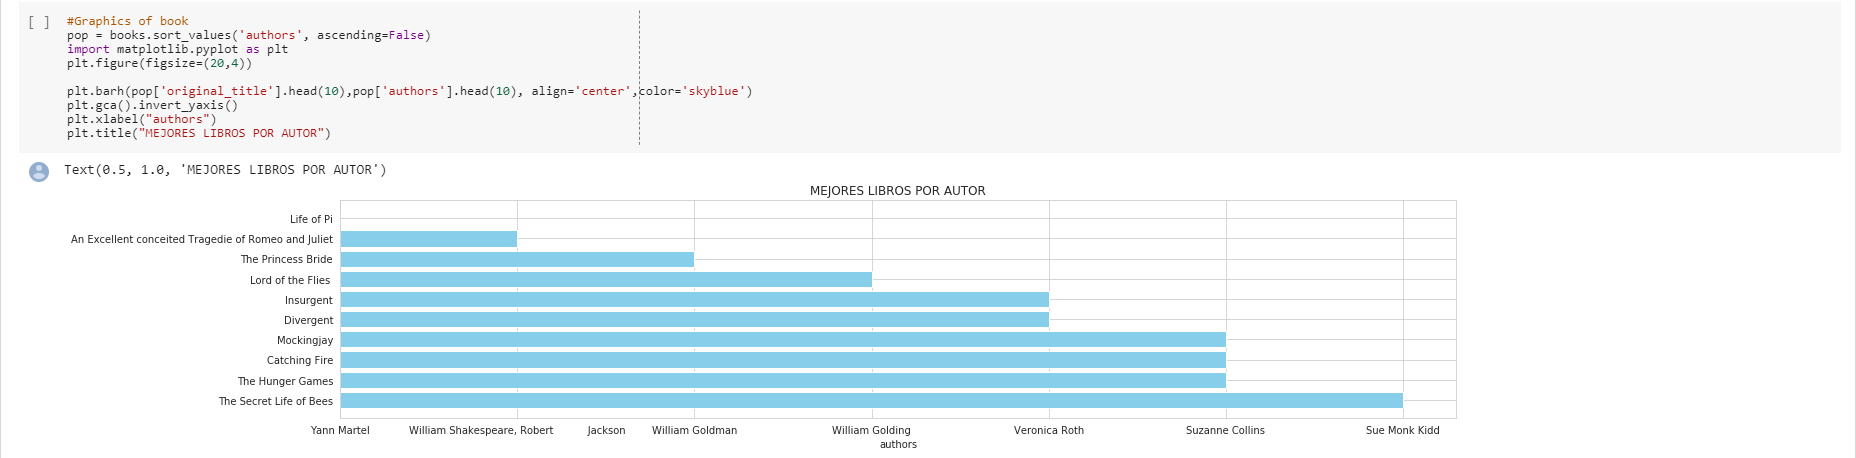
\includegraphics[scale= 0.40]{./Imagenes/mejores_libros_p_autor.png}
\end {center}


\item Consultas de Mejores Libros por Rating 1

Este objetivo se hace necesario para poder iniciar una valoracion de los libros.

\begin {center}
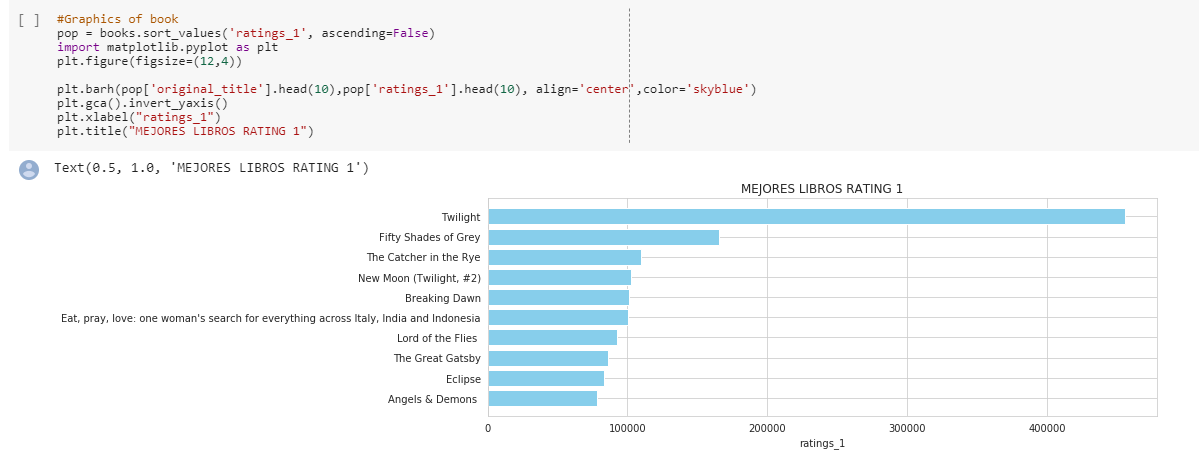
\includegraphics[scale= 0.50]{./Imagenes/mejores_libros_rating_1.png}
\end {center}


\end{itemize}


\section{Conclusion}
El método Kimball está orientado a la consulta de la información, por lo que su estructura interna está especialmente diseñada para garantizar una explotación de los datos rápida y sencilla, no requiriendo usuarios especializados para ello. Por el contrario, el método Inmon persigue la integración de todos los datos de la compañía, estando orientado hacia el almacenaje de grandes volúmenes de datos, por lo que su estructura interna normalizada se diseña para evitar la redundancia de datos, simplificar las labores de mantenimiento, etc. cuestiones que complican las consultas de la información, requiriendo que los usuarios finales estén mucho más especializados.
Así, podríamos decir que el enfoque de Kimball se ajusta más a proyectos pequeños en los que se persiga un sistema fácilmente explotable y entendible por el usuario y de rápido desarrollo, siendo el modelo de Inmon más apropiado para sistemas complejos de mayor importancia.

%%
	
	%%
	%\linenumbers
	
	%% main text

	
	
	\newpage
	
		%ESTILO
	   \bibliography{BIBLIOGRAFIA}		%ARCHIVO .bib
	   \begin{thebibliography}{0}
              \bibitem{Ronald} 
 	    \bibitem{Angelo} 
                 \bibitem{Juan} http://tdan.com/data-warehouse-design-inmon-versus-kimball/20300
                  \bibitem{Jhordy} https://blog.bi-geek.com/arquitectura-comparativa-inmon-y-kimball/
                  \bibitem{Jhordy} https://churriwifi.wordpress.com/2010/04/19/15-2-ampliacion-conceptos-del-modelado-dimensional/
                    \bibitem{Brandon} https://twooctobers.com/blog/8-data-storytelling-concepts-with-examples/
                   \bibitem{Brandon}https://www.ucasal.edu.ar/htm/ingenieria/cuadernos/archivos/5-p56-rivadera-formateado.pdf

         \end{thebibliography}
	
\end{document}

%%
%% End of file `elsarticle-template-1-num.tex'.
